\section{Auswertung}

\subsection{Amplitudenmodulation mit Ringmodulator}

Mit dem Ringmodulator wird die Amplitude eines Signals moduliert. Das Eingans- und Ausgangssignal sind in \autoref{a} zu sehen. Das Trägersignal hatte eine Amplitude von $U_\text{T}=\SI{0}{\volt}$ und die Frequenz $\omega_\text{T}=\SI{0}{\hertz}$, das Modulationssignal hatte eine Amplitude von $U_\text{M}=\SI{0}{\volt}$ und die Frequenz $\omega_\text{M}=\SI{0}{\hertz}$. Es entsteht eine Schwebung, die Trägerfrequenz ist hier nicht zu erkennen. Die prominentesten Linien in dem Frequenzspektrum in \autoref{b} sind die der Modulationsfrequenz. Dazwischen ist als kleinerer Peak auch die Trägerfrequenz zu sehen, die mit dem Ringmodulator nicht komplett unterdrückt wird, aber signifikant kleiner als die Seitenbänder ist.

\begin{figure}
	\centering
	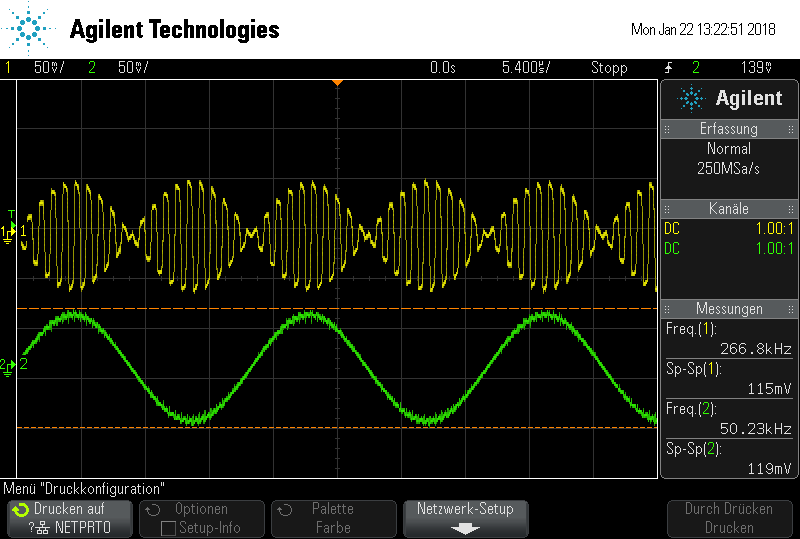
\includegraphics[width=\textwidth]{img/a_scope_230.png}
	\caption{Amplitudenmodulation - grün das Eingangssignal, gelb das amplitudenmodulierte Signal}
	\label{a}
\end{figure}

\begin{figure}
	\centering
	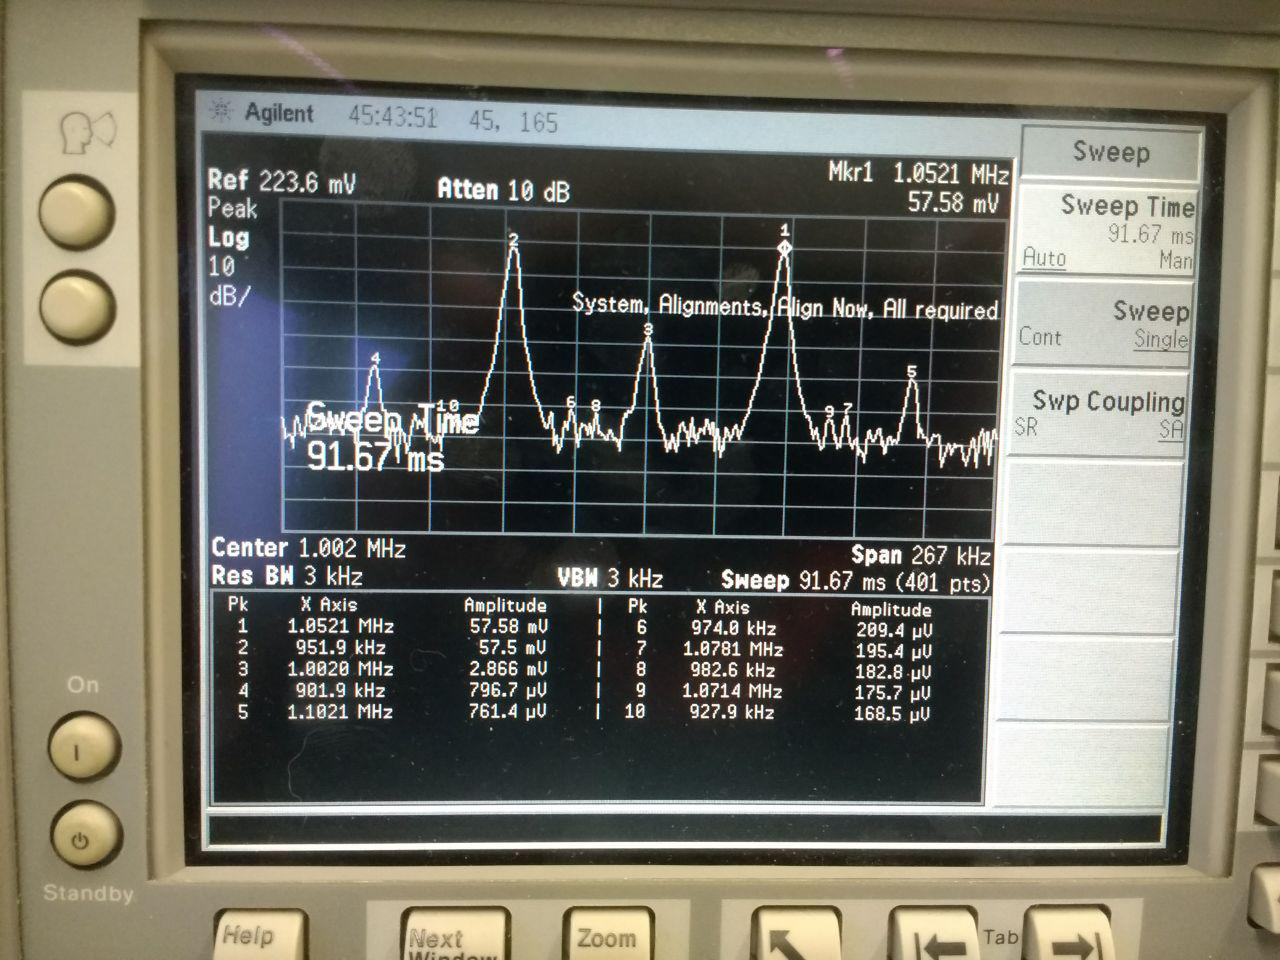
\includegraphics[width=\textwidth]{img/Aufgabenteil_b.jpg}
	\caption{Amplitudenmodulation - Peak 3 mit der Trägerfrequenz, Peak 1 und 2 die Seitenbänder}
	\label{b}
\end{figure}

\subsection{Amplitudenmodulation mit Trägerabstrahlung}

In \autoref{c1} ist das Fequenzspektrum einer amplitudenmodulierten Schwingung mit Trägerabstrahlung zu sehen. Das Trägersignal hatte eine Amplitude von $U_\text{T}=\SI{0}{\volt}$ und die Frequenz $\omega_\text{T}=\SI{0}{\hertz}$, das Modulationssignal hatte eine Amplitude von $U_\text{M}=\SI{0}{\volt}$ und die Frequenz $\omega_\text{M}=\SI{0}{\hertz}$. \autoref{c2} zeigt von dem gleichen Signal eine Oszilloskop-Aufnahme. In \autoref{c2} lässt sich der Modulationsgrad aus dem Verhältnis der Amplitude der Maxima und der Minima bestimmen. Da die Amplitude zwischen $U_\text{min} = U_\text{T}(1 - m)$ und $U_\text{max} = U_\text{T}(1 + m)$ schwankt, ist der Modulationsgrad
\[
	m =\frac{U_\text{max} - U_\text{min}}{U_\text{max} + U_\text{min}} = \frac{\SI{52}{\milli\volt} - \SI{26}{\milli\volt}}{\SI{52}{\milli\volt} + \SI{26}{\milli\volt}} = 0.33.
\]
Eine andere Methode, den Modulationsgrad zu bestimmen, ist mit der Peakhöhe der Träger- und Modulationsfrequenz im Frequenzanalysator.
\[
	m_1 = 4 \cdot \frac{10^{-44.62/10}}{10^{-33.68/10}} = 0.322, \quad m_2 = 4 \cdot \frac{10^{-44.7/10}}{10^{-33.68/10}} = 0.316
\]

\begin{figure}
	\centering
	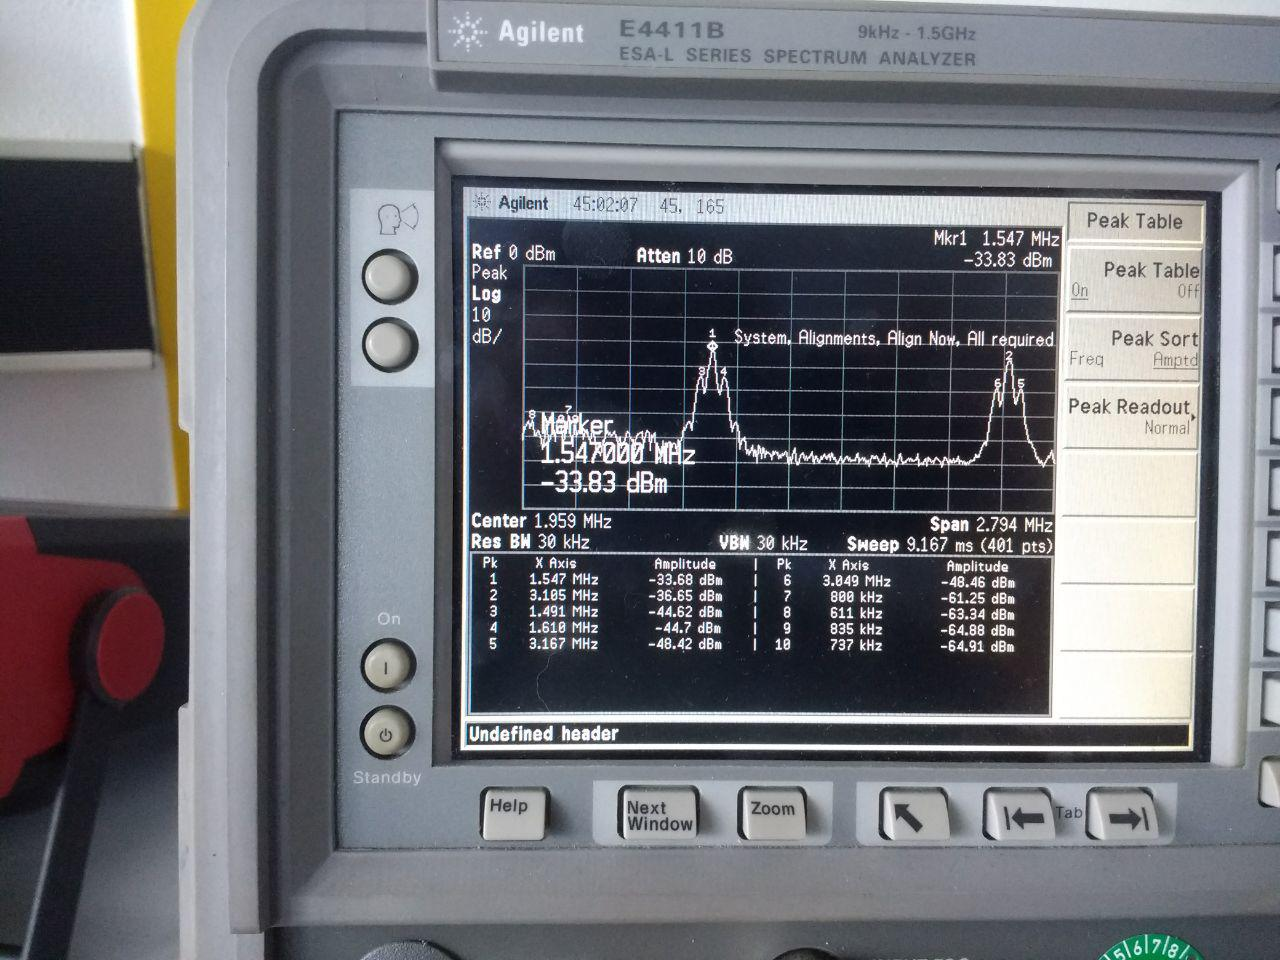
\includegraphics[width=\textwidth]{img/Aufgabenteil_c1.jpg}
	\caption{Amplitudenmodulation mit Oberwellen, Trägerabstrahlung und Seitenbändern}
	\label{c1}
\end{figure}

\begin{figure}
	\centering
	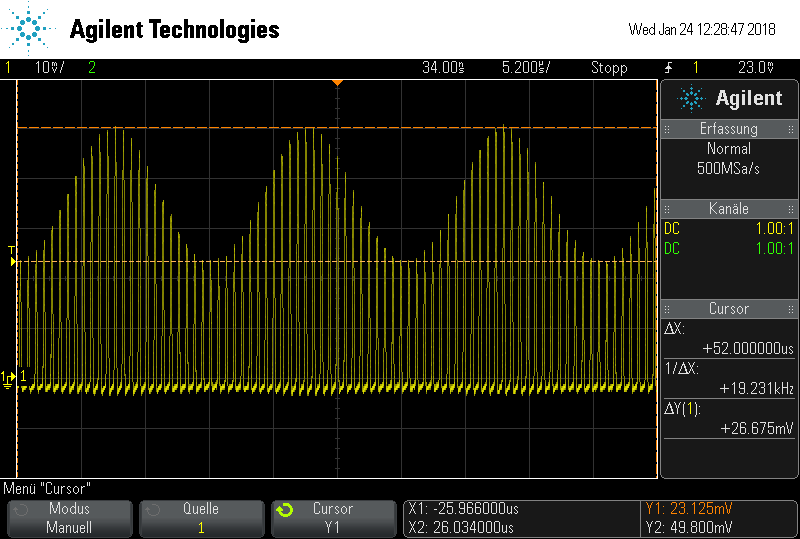
\includegraphics[width=\textwidth]{img/c_scope_247.png}
	\caption{Amplitudenmodulation - Bestimmung des Modulationsgrades}
	\label{c2}
\end{figure}

\begin{figure}[t!]
	\centering
	\begin{subfigure}[t]{0.5\textwidth}
		\centering
		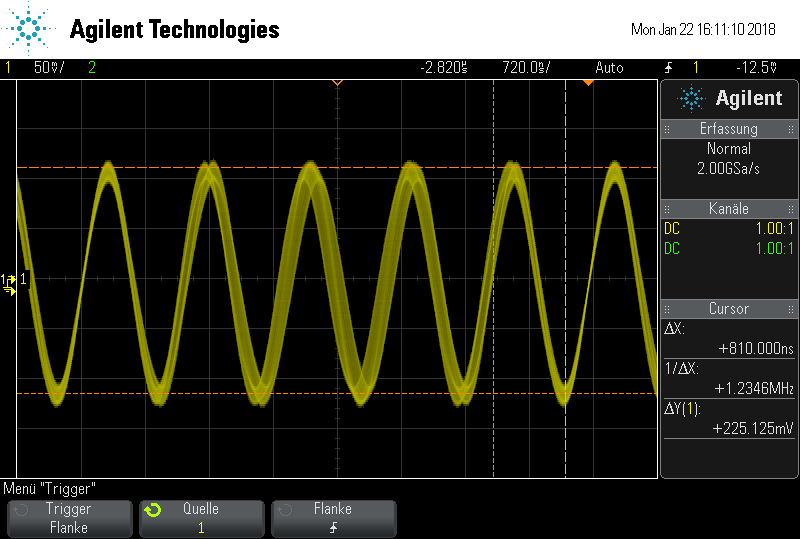
\includegraphics[width=\textwidth]{img/d_scope_233.png}
		\caption{Frequenzmodulation}
	\end{subfigure}%
	~
	\begin{subfigure}[t]{0.5\textwidth}
		\centering
		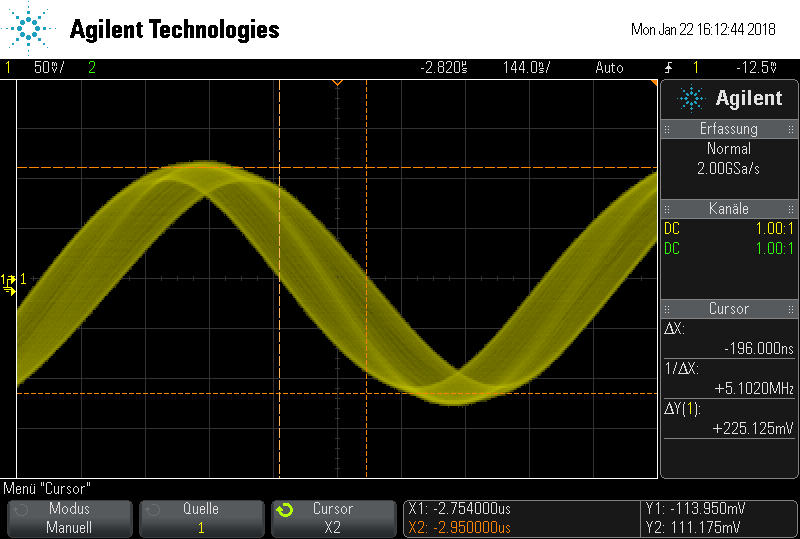
\includegraphics[width=\textwidth]{img/d_scope_234.png}
		\caption{Frequenzmodulation - Detailansicht}
	\end{subfigure}
\end{figure}

\begin{figure}
	\centering
	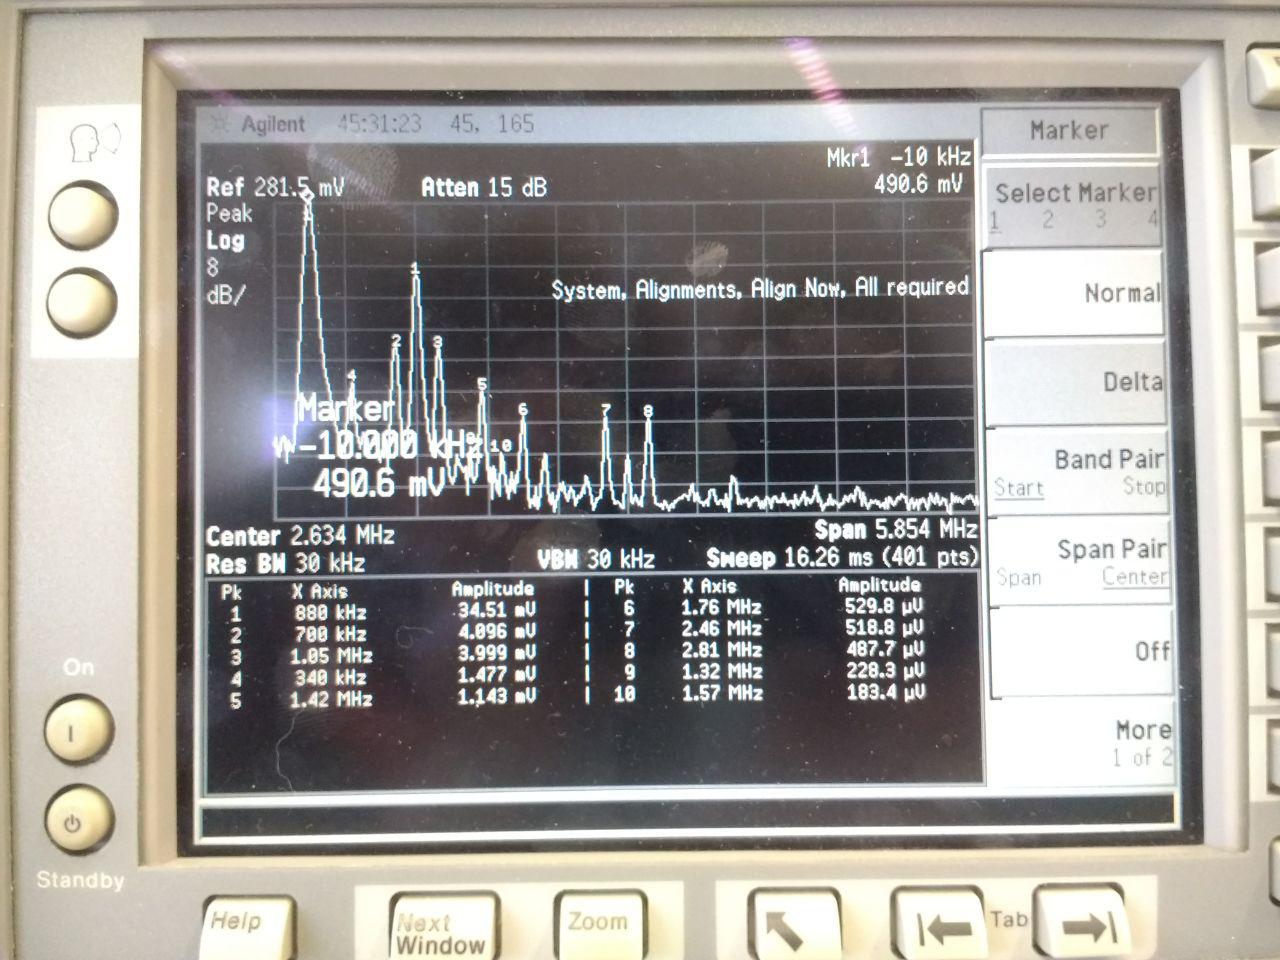
\includegraphics[width=\textwidth]{img/Aufgabenteil_d.jpg}
	\caption{Frequenzmodulation - Frequenzspektrum}
\end{figure}

\subsection{Demodulation mit Ringmodulator}

%Tabelle \autoref{tab:e} mit Messwerten und Ausgleichsrechnung \autoref{fig:e}

In \autoref{f} ist die Oszilloskop-Aufnahme eines Signals zu sehen, dessen Amplitude zunächst moduliert und daraufhin wieder demoduliert wird. In gelb ist das Eingangssignal, die grüne Kurve ist das um einen festen Faktor phasenverschobene und in der Amplitude reduzierte Signal.

\begin{figure}
	\centering
	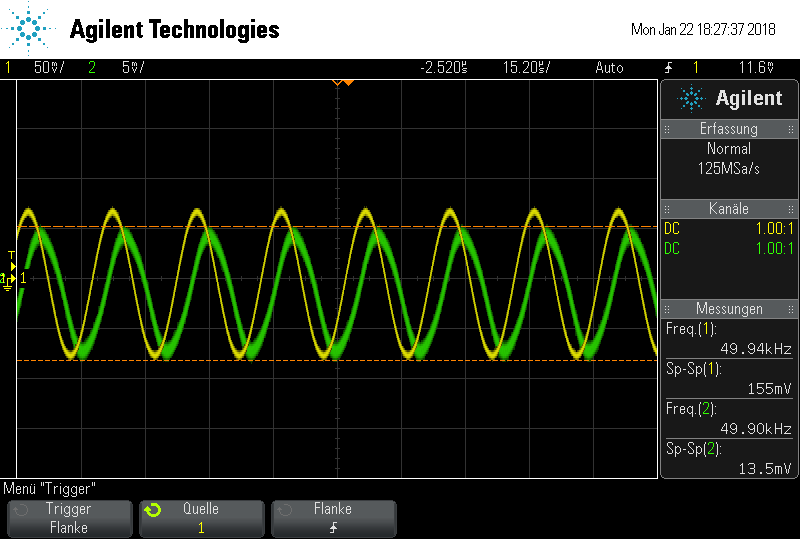
\includegraphics[width=\textwidth]{img/f_scope_235.png}
	\caption{Amplituden(de-)modulation - gelb das Eingangssignal, grün das amplitudenmodulierte und daraufhin demodulierte Signal}
	\label{f}
\end{figure}

\subsection{Demodulation mit Gleichrichterdiode}

\begin{figure}[t!]
	\centering
	\begin{subfigure}[t]{0.5\textwidth}
		\centering
		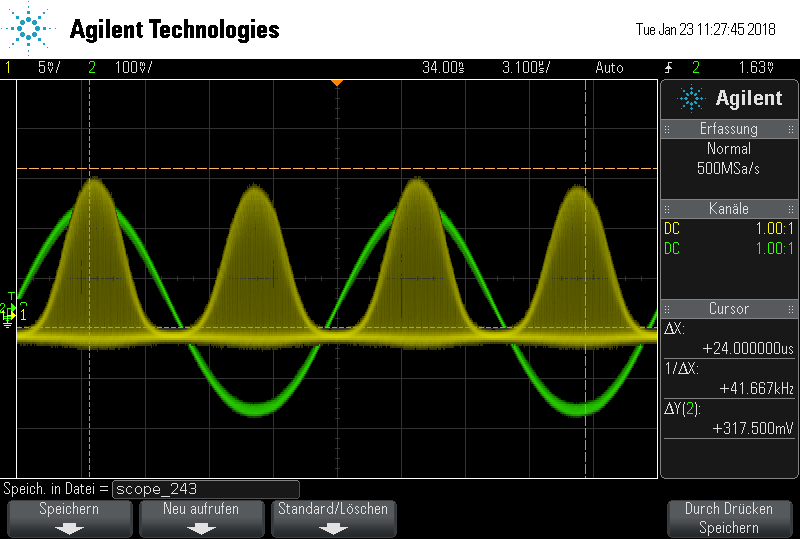
\includegraphics[width=\textwidth]{img/g_scope_243.png}
		\caption{Frequenzmodulation}
	\end{subfigure}%
	~
	\begin{subfigure}[t]{0.5\textwidth}
		\centering
		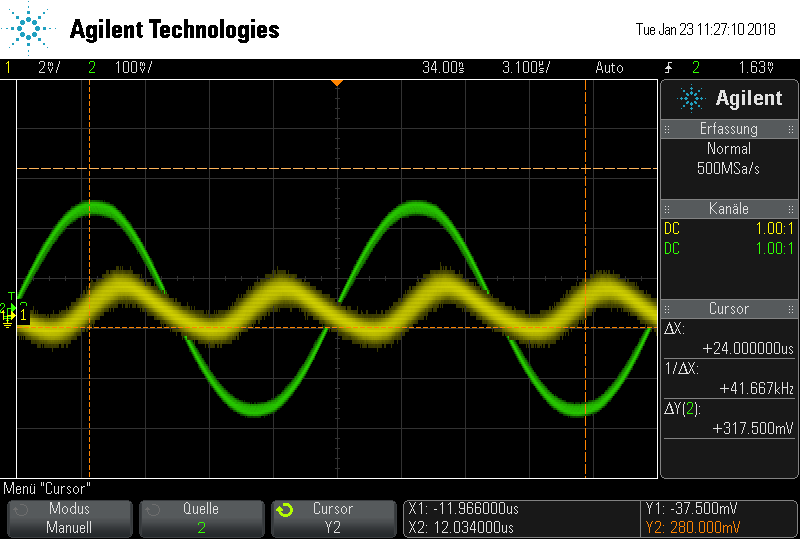
\includegraphics[width=\textwidth]{img/g_scope_242.png}
		\caption{Frequenzmodulation - Detailansicht}
	\end{subfigure}
\end{figure}

\subsection{Demodulation einer frequenzmodulierten Schwingung}

\begin{figure}[t!]
	\centering
	\begin{subfigure}[t]{0.5\textwidth}
		\centering
		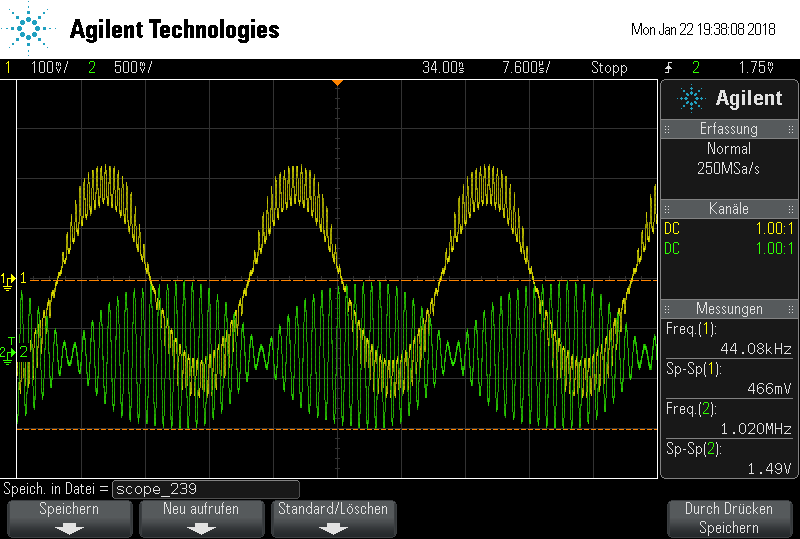
\includegraphics[width=\textwidth]{img/h_scope_239.png}
		\caption{Amplitudenmodulation - Amplitudenmodulation - moduliertes  Signal in grün, Eingangssignal in gelb}
	\end{subfigure}%
	~
	\begin{subfigure}[t]{0.5\textwidth}
		\centering
		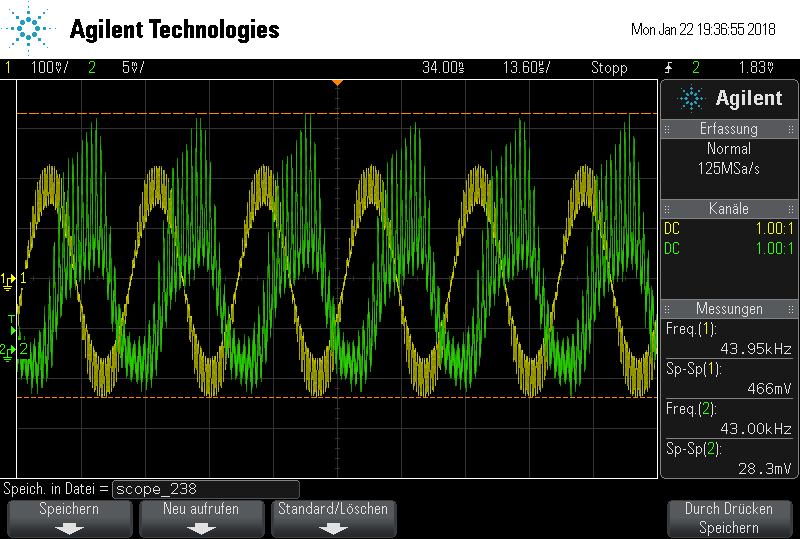
\includegraphics[width=\textwidth]{img/h_scope_238.png}
		\caption{Amplitudenmodulation - moduliertes und dann demoduliertes Signal in grün, Eingangssignal in gelb}
	\end{subfigure}
	\\
	\begin{subfigure}[t]{0.5\textwidth}
		\centering
		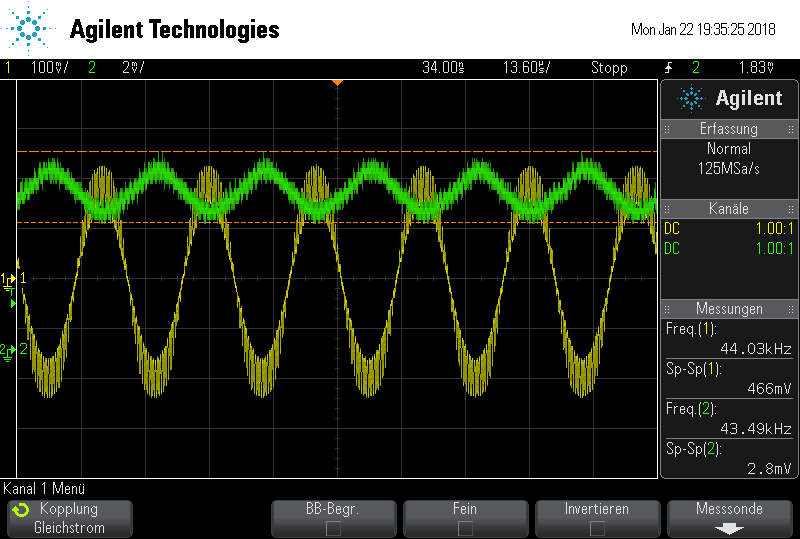
\includegraphics[width=\textwidth]{img/h_scope_237.png}
		\caption{Amplitudenmodulation - moduliertes und dann demoduliertes Signal nach Hochpass in grün, Eingangssignal in gelb}
	\end{subfigure}
\end{figure}

\FloatBarrier
